\section{Deadlock}
Quando due processi richiedono la stessa risorsa non condivisibile, uno dei due attende l'altro.

\spacer
In alcuni casi però si può arrivare ad una situazione più complicata, ovvero quando due o più processi si attendono a vicenda, questo viene detto \textbf{deadlock} o \textbf{stallo}.

\spacer
Le condizioni necessarie (ma non sufficienti) per il verificarsi di un \textbf{deadlock}:
\begin{enumerate}
    \item Tutte le risorse devono essere non condivisibili.
    \item Il processo non ha un'unica operazione in cui richiede delle risorse.
    \item Al processo non può essere rimossa la risorsa, solo esso stesso può rilasciarla.
    \item L'attesa avviene in modo circolare, se ci sono $n$ processi, $P_1$ attende $P_2$, $\ldots$, $P_(n-1)$ attende $P_n$ e $P_n$ attende $P_1$.
\end{enumerate}

In questo caso ogni processo attende una risorsa che non verrà rilasciata, tutti attendono e nessuno può procedere.

\subsubsection*{Livelock}
Un sottoinsieme dei deadlock sono i livelock o stalli attivi, rappresenta una situazione dove i thread non sono effettivamente bloccati, ma effettivamente non progrediscono (es. due persone che si incontrano e si spostano ripetutamente da un lato all'altro del corridoio)

\subsection{Grafo delle Risorse}
Una visualizzazione utile per evidenziare possibili deadlock in fase di progettazione è il grafo delle risorse.

\spacer
I nodi del grafo rappresentano thread ($T_1, T_2, \ldots, T_n$) e risorse ($R_1, R_2, \ldots, R_n$), spesso vengono visualizzati in modo differente per distinguerli.

Diciamo \textit{arco di richiesta} $T_i -> R_j$ e un \textit{arco di assegnazione} $R_i -> T_j$

\spacer
A questo punto possiamo dire che se il grafo non contiene cicli chiusi allora non ci saranno deadlock. Quando invece il grafo contiene un ciclo e vi è una sola istanza per ogni risorsa allora ci sarà un deadlock, se almeno una risorsa ha più di un'istanza allora il deadlock è solamente possibile.

\begin{figure}[H]
    \centering
    \begin{minipage}{0.45\textwidth}
        \centering
        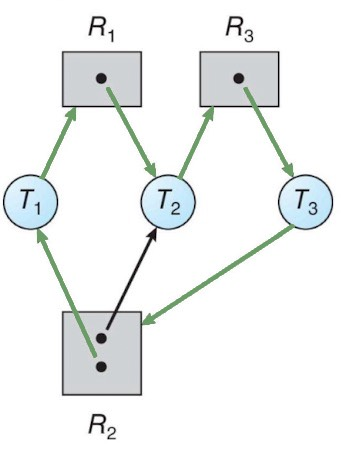
\includegraphics[width=0.65\linewidth]{assets/ciclo-deadlock.jpg}
        \caption{Situazione di deadlock}
    \end{minipage}
    \hfill
    \begin{minipage}{0.45\textwidth}
        \centering
        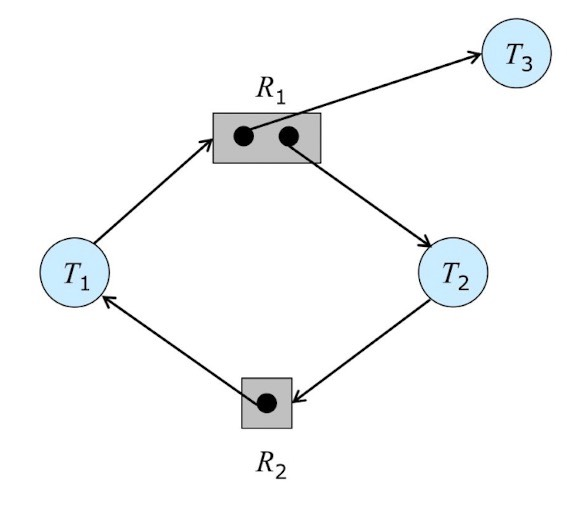
\includegraphics[width=0.9\linewidth]{assets/ciclo-no-deadlock.jpg}
        \caption{Situazione priva di deadlock}
    \end{minipage}
\end{figure}

\subsection{Prevenzione dei Deadlock}

\subsubsection{Allocazione globale}
Tutte le risorse richieste da un processo devono essere allocate prima che inizi l'esecuzione.

Questo garantisce l'assenza di deadlock, tuttavia è estremamente inefficiente reclamare tutte le risorse per tutto il periodo di esecuzione.

\subsubsection{Allocazione gerarchica}
Si assegna un ordine di importanza alle risorse, un processo può richiedere solo risorse più elevate di quelle che ha attualmente.
Se un processo necessita di una risorsa di priorità inferiore deve rilasciare quella attualmente in suo possesso per poi tornare a richiederla.

\begin{minipage}{0.45\textwidth}
    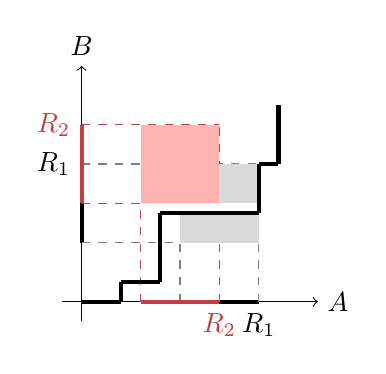
\begin{tikzpicture}[scale=2.5]
        % assi
        \draw[->] (-0.1,0) -- (1.2,0) node[right] {$A$};
        \draw[->] (0,-0.1) -- (0,1.2) node[above] {$B$};

        %R1
        \draw[smooth, line width=1.5pt] (0, 0.3) -- (0, 0.7) node[left] {$R_1$};
        \draw[smooth, line width=1.5pt] (0.5, 0) -- (0.9, 0) node[below] {$R_1$};


        \draw[dashed, gray] (0, 0.3) -- (0.5, 0.3);
        \draw[dashed, gray] (0, 0.7) -- (0.9, 0.7);

        \draw[dashed, gray] (0.5, 0) -- (0.5, 0.3);
        \draw[dashed, gray] (0.9, 0) -- (0.9, 0.7);

        %R2
        \draw[smooth, line width=1.5pt, red!50!gray] (0, 0.5) -- (0, 0.9) node[left] {$R_2$};
        \draw[smooth, line width=1.5pt, red!50!gray] (0.3, 0) -- (0.7, 0) node[below] {$R_2$};


        \draw[dashed, red!40!gray] (0, 0.5) -- (0.3, 0.5);
        \draw[dashed, red!40!gray] (0, 0.9) -- (0.7, 0.9);

        \draw[dashed, red!40!gray] (0.3, 0) -- (0.3, 0.5);
        \draw[dashed, red!40!gray] (0.7, 0) -- (0.7, 0.9);

        %squares
        \draw[fill=gray!30, draw=none] (0.5,0.3) rectangle (0.9, 0.7);
        \draw[fill=red!30, draw=none] (0.3,0.5) rectangle (0.7, 0.9);
        \draw[fill=white, draw=none] (0.3,0.45) rectangle (0.9, 0.5);

        % grafico
        \draw[smooth, line width=1.5pt] (0, 0) -- (0.2, 0);
        \draw[smooth, line width=1.5pt] (0.2, 0) -- (0.2, 0.1);
        \draw[smooth, line width=1.5pt] (0.2, 0.1) -- (0.4, 0.1);
        \draw[smooth, line width=1.5pt] (0.4, 0.1) -- (0.4, 0.45);
        \draw[smooth, line width=1.5pt] (0.4, 0.45) -- (0.9, 0.45);
        \draw[smooth, line width=1.5pt] (0.9, 0.45) -- (0.9, 0.7);
        \draw[smooth, line width=1.5pt] (0.9, 0.7) -- (1, 0.7);
        \draw[smooth, line width=1.5pt] (1, 0.7) -- (1, 1);
    \end{tikzpicture}
\end{minipage}

\subsubsection{Algoritmo del Banchiere}
Si impone che il thread $T_i$ inserisca nel grafo delle risorse tutti gli \textbf{archi di reclamo} a lui necessari prima di iniziare l'esecuzione.

Un arco di reclamo di un thread verso una risorsa indica al sistema che il thread utilizzerà in futuro quella risorsa. Un arco di reclamo diventa poi arco di richiesta in futuro.

\spacer
Definiamo \textbf{sequenza sicura} un ordinamento di n processi tali per lui le richieste di $P_i$ siano soddisfacibili dai processi $P_j$ con $j<i$

Uno \textbf{stato sicuro} è uno stato che contiene almeno una sequenza sicura.

\spacer
Per implementare l'algoritmo del banchiere vanno mantenute diverse strutture dati:
\begin{sitemize}
    \item Un \textbf{vettore $V$} che contiene il numero di istanze disponibili per ogni risorsa.
    \item Una \textbf{matrice $M$} che memorizza la massima quantità di istanze per ogni risorsa che viene usata dal thread.
    \item Una \textbf{matrice $R$} che memorizza le istanze per ogni risorsa attualmente allocate ad ogni thread.
    \item Una \textbf{matrice $N = M - R$}, che memorizza le risorse mancanti ad ogni thread.
\end{sitemize}

Tutte queste matrici devono essere aggiornate sia nei valori che nelle dimensioni.

\spacer
Per verificare che lo stato corrente sia sicuro deve essere possibile trovare almeno una sequenza di processi tale per cui sia possibile assegnare le risorse del vettore per completare ogni processo (le risorse necessarie al processo $i$ si trovano su $N[i]$)

\subsubsection{Algoritmo dello Struzzo}
L'algoritmo del banchiere deve essere eseguito frequentemente per poter rilevare i deadlock prima che si rivelino problematici, questo però richiede parecchie risorse del sistema.

\spacer
Per questo motivo molti sistemi \textit{consumer} \textbf{non} gestiscono i deadlock, essi avvengono in media una volta l'anno e in quel caso il sistema dovrà essere riavviato.

\subsection{Risoluzione di un Deadlock}
Una volta rilevato un deadlock per risolverlo ci sono due strategie spesso utilizzate.

\subsubsection{Terminazione dei Processi}
\begin{sitemize}
    \item Terminazione di tutti i processi che fanno parte del deadlock.

    Un sistema che risolve sicuramente il deadlock, ma viene anche ad un gran costo computazionale in quanto tutti i processi dovranno venir eseguiti da zero.

    \item Terminazione di un processo per volta finché il deadlock non viene rotto.
\end{sitemize}

\spacer
La scelta del processo da terminare è anch'essa gestita da un algoritmo che prende in considerare molti fattori, come la priorità del thread, il tempo di computazione trascorso, quantità di risorse che utilizza.


\subsubsection{Prelazione di Risorse}
Per risolvere il deadlock è anche possibile rimuovere risorse forzatamente ad uno o più processi.

Alcuni fattori da considerare quando si applica questa strategia sono:
\begin{sitemize}
    \item \textbf{Selezione della vittima}, è necessario scegliere un processo a cui rimuovere le risorse.
    \item \textbf{Rollback} dopo la rimozione della risorsa il thread non può continuare la sua esecuzione, è necessario tornare indietro a quando quella risorsa è stata acquisita.
    \item \textbf{Starvation} è importante non prelare le risorse sempre dallo stesso processo, altrimenti si potrebbe arrivare alla situazione in cui un processo non procede mai.
\end{sitemize}